% ======================================================================
%  ABLATION STUDIES
% ======================================================================
\section{Ablation Studies}\label{sec:ablation}

\subsection{Confidence Filter}

The $|\hat{z}| \geq 0.5$ confidence filter restricts trading to high-confidence predictions. Table~\ref{tab:filter_ablation} quantifies its effect on R$^2$.

\begin{table}[h]
\caption{Effect of the $|\hat{z}| \geq 0.5$ confidence filter on model R$^2$ across campaigns.}
\label{tab:filter_ablation}
\small
\begin{tabular}{lrrrr}
\toprule
\textbf{Campaign} & \textbf{All R$^2$} & \textbf{Filtered R$^2$} & \textbf{$\Delta$} & \textbf{\% rows filtered} \\
\midrule
Jul~30 (live)  & 0.054 & 0.248 & +0.194 & 10.3\% \\
Jul~31 (live)  & 0.104 & 0.347 & +0.243 & 14.9\% \\
Offline test   & 0.133 & 0.383 & +0.250 & --- \\
\bottomrule
\end{tabular}
\end{table}

The filter consistently lifts R$^2$ by approximately 0.2--0.25 across all evaluation settings, as shown in Figure~\ref{fig:filter_lift}. Importantly, this lift is not free: the filtered subset constitutes only 10--15\% of all predictions, meaning 85--90\% of snapshot/pair observations are declined. The filter strategy parallels the ``skip low-magnitude predictions'' approach shown to improve profit-per-trade in Sarmento et al.~\cite{sarmento2024ml}.

\begin{figure}[h]
\centering
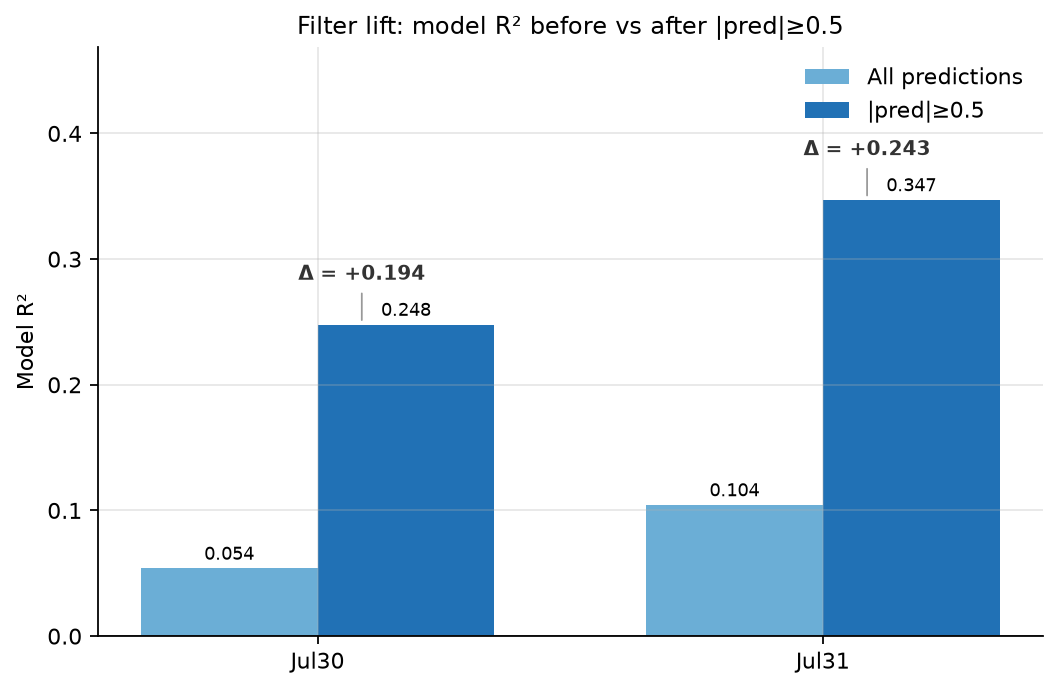
\includegraphics[width=\columnwidth]{figures/fig3_filter_r2_lift.png}
\caption{Model R$^2$ before and after the $|\hat{z}| \geq 0.5$ confidence filter. The filter selects predictions in high-signal regimes, lifting R$^2$ by +0.19 to +0.25 across both live campaigns.}
\Description{Grouped bar chart of model R squared on a vertical axis from zero to
0.35 for the two live campaigns. For Jul 30 the all-predictions bar is 0.054 and
the filtered bar is 0.248, a rise of 0.194. For Jul 31 the all-predictions bar is
0.104 and the filtered bar is 0.347, a rise of 0.243. In both campaigns the
filtered bar is roughly three times the height of the unfiltered bar.}
\label{fig:filter_lift}
\end{figure}

A critical caveat: much of the filtered directional accuracy is explained by persistence in high-$|z|$ states rather than incremental model skill. On Jul~31 filtered rows, naive persistence achieves 77.0\% directional accuracy versus the model's 76.7\%. The model's advantage is in R$^2$ (0.347 vs 0.174), indicating that it captures the \emph{magnitude} of future z-score movements more accurately than simply predicting that large z-scores will persist.

\subsection{Feature Importance: Role of Microstructure Inputs}

Figure~\ref{fig:importance} shows the top~20 of the model's 68~features by LightGBM split gain.

\begin{figure}[h]
\centering
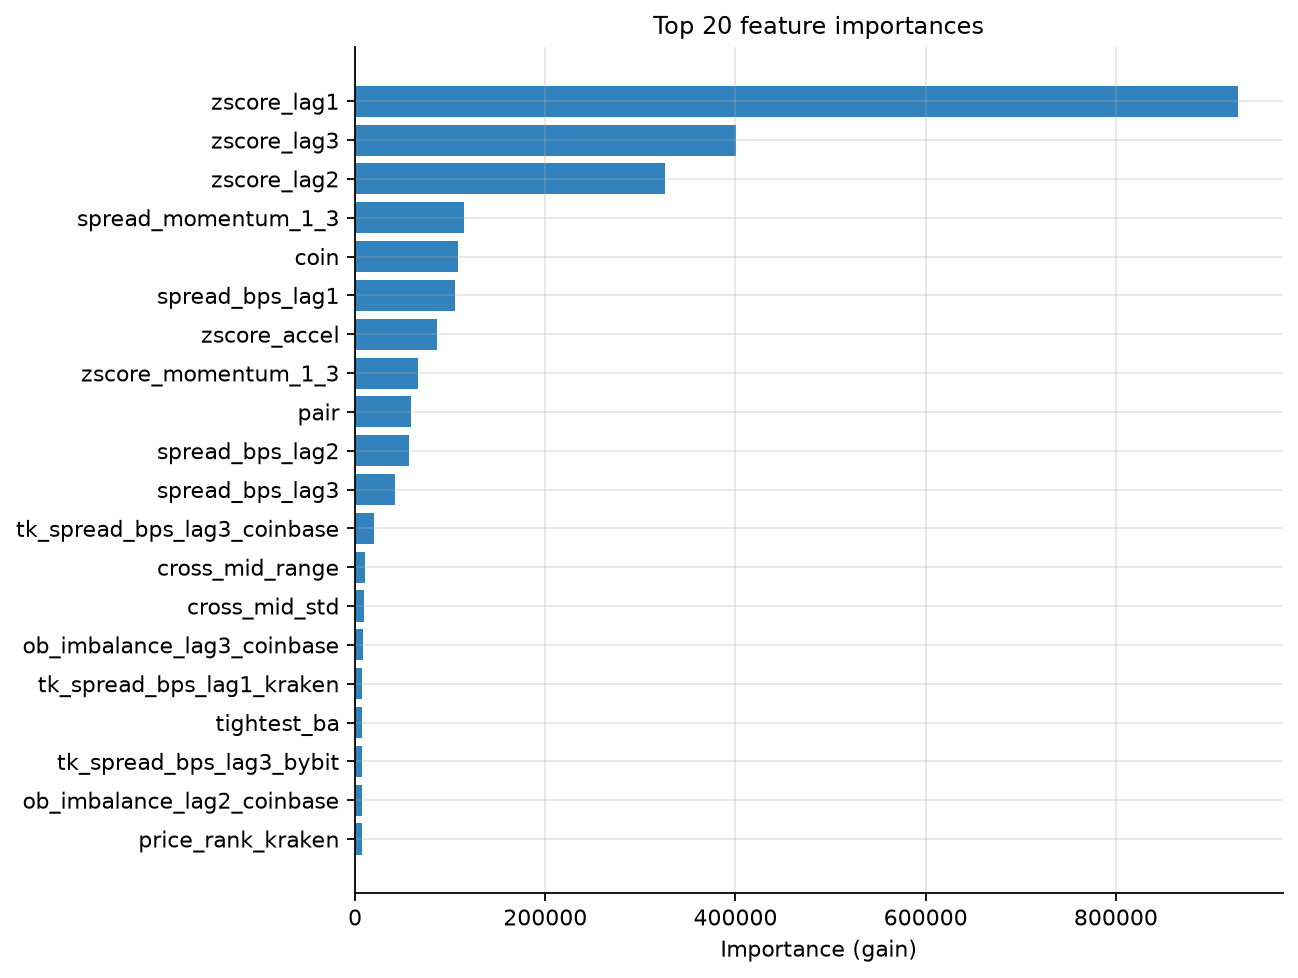
\includegraphics[width=\columnwidth]{figures/fig4_feature_importance_top20.png}
\caption{Top~20 features by LightGBM split gain. Gain is overwhelmingly
concentrated in the lagged z-score and spread terms; microstructure features
enter only in the lower half of the ranking.}
\Description{Horizontal bar chart of the twenty highest-gain features, ordered
from largest at the top. The first bar, lagged z-score at lag one, reaches about
930,000 gain. Lagged z-score at lags three and two follow at about 400,000 and
325,000. Spread momentum, the coin categorical, lagged spread in basis points,
z-score acceleration, z-score momentum, the pair categorical, and two further
lagged spread terms range from about 115,000 down to 42,000. The remaining nine
bars are all below about 20,000 and are visually near-zero against the first bar;
they comprise per-venue bid-ask spread lags for Coinbase, Kraken and Bybit,
cross-venue mid-price range and standard deviation, two Coinbase orderbook
imbalance lags, the tightest bid-ask indicator, and a Kraken price rank.}
\label{fig:importance}
\end{figure}

The model is, to a first approximation, an autoregression on the recent z-score trajectory conditioned on asset and venue-pair identity, with microstructure features supplying a small correction. Lagged z-scores and spread dynamics dominate the top~10 by split gain; microstructure and cross-venue dispersion features (per-venue bid-ask spreads, orderbook imbalance, \texttt{cross\_mid\_range}) enter only in the lower half of the ranking. Only two of the twenty highest-gain features are orderbook imbalance terms, and no trade-flow, funding-rate, or open-interest feature appears in the top~20. The cross-venue dispersion and orderbook features are genuinely unavailable to single-venue or backtest-only systems, but establishing their marginal contribution to R$^2$ requires a leave-one-group-out retraining study that we have not run.

